% !TeX root = ../../main.tex
\section{Evaluation}
\label{sec:evaluation}

% Draft from the outline: Evaluation. Subsection names follow the outline.

\subsection{Perturbation Study}
\label{sec:perturbation}

\begin{figure*}[t]
  \centering
  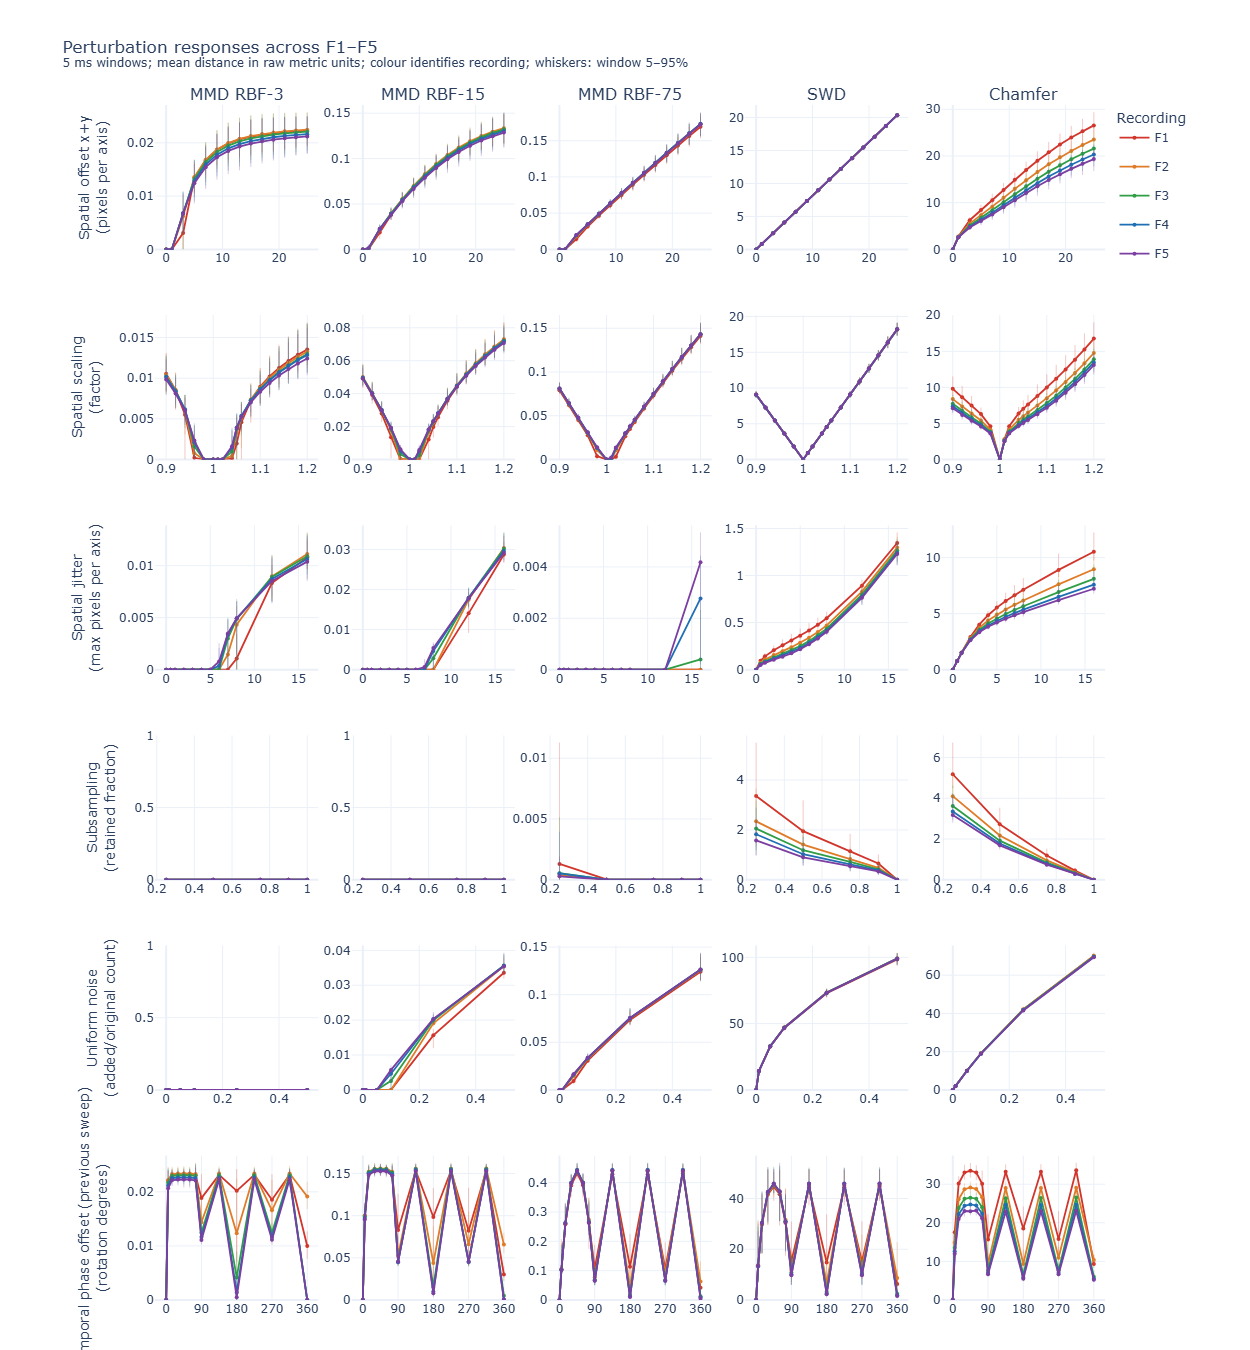
\includegraphics[width=\textwidth]{paper/Images/Perturbation_figure_all.png}
  \caption[Perturbation responses]{\todo{Caption for the combined perturbation figure.}}
  \label{fig:perturbation-responses}
\end{figure*}

\todo{Uncertainty of the perturbation responses (the whole-recording noise floor run can serve as the basis).}

\subsubsection{Spatial Translation and Spatial Scaling}
\label{sec:translation-scaling}

\subsubsection{Spatial Jitter}
\label{sec:jitter}

\subsubsection{Subsampling}
\label{sec:subsampling}

\subsubsection{Uniform Noise}
\label{sec:noise}

\subsubsection{Temporal Offset}
\label{sec:temporal-offset}

\subsubsection{Summary of Perturbation Responses}
\label{sec:perturbation-summary}

\subsection{Simulator Study}
\label{sec:simulator}

\subsubsection{Comparison Setup}
\label{sec:simulator-setup}

\todo{Noise floor: the 360-degree point of the temporal offset test for now; the whole-recording run is the alternative.}

\subsubsection{v2e}
\label{sec:v2e}

\todo{One sentence on timing: v2e matches real best when shifted by +3 to +7 ms.}

\subsubsection{V2CE}
\label{sec:v2ce}

\subsubsection{Example Study}
\label{sec:example-study}

\todo{Parameter tuning example promised in the introduction.}
